

\documentclass{beamer}
\mode<presentation> {

\usetheme{Boadilla}

}

\usepackage{graphicx} % Allows including images
\usepackage{booktabs} % Allows the use of \toprule, \midrule and \bottomrule in tables
\usepackage[export]{adjustbox} %positioning of graphics
%\usepackage{threeparttable} 
%\usepackage[labelformat=empty,font=scriptsize,skip=0pt,
%justification=raggedright,singlelinecheck=false]{caption}

\usepackage{caption}
\captionsetup[figure]{justification=raggedright,singlelinecheck=false} %rightalign
\captionsetup{font=scriptsize,labelfont=scriptsize} %change fontsize
\setbeamertemplate{caption}[numbered] % numerate figures

\title[Exocentric Pointing in Virtual Reality]{Exocentric Pointing in Virtual Reality:\\ Measuring the Intrinsic Geometry of the Visual Space} % The short title appears at the bottom of every slide, the full title is only on the title page
\subtitle{Final Presentation on my Bachelor Thesis} %not ideal
\author{Rahel Gerrens} % Your name
%\institute[UCLA] % Your institution as it will appear on the bottom of every slide, may be shorthand to save space
%{
%University of California \\ % Your institution for the title page
%\medskip
%\textit{john@smith.com} % Your email address
%}
\date{19.10.2020} % Date, can be changed to a custom date

%%%%%%%%%%%%%%%%%
\begin{document}

\begin{frame}
\titlepage % Print the title page as the first slide
\end{frame}

%\begin{frame}
%\frametitle{Overview} % Table of contents slide, comment this block out to remove it
%\tableofcontents % Throughout your presentation, if you choose to use \section{} and \subsection{} commands, these will automatically be printed on this slide as an overview of your presentation
%\end{frame}

\section{Background}

\begin{frame}{Luneburg (1947)}
    \begin{itemize}
        \item Theoretical analysis of the visual space 
        \item The visual space has a hyperbolic curvature ($K< 0$)
        \item The curvature is constant
        \item Empirical evidence for theory given by many experiments
    \end{itemize}
\end{frame}

\begin{frame}{Koenderink et al. (2000)}
    \begin{minipage}{5cm}
        \begin{figure}
            \raggedright
            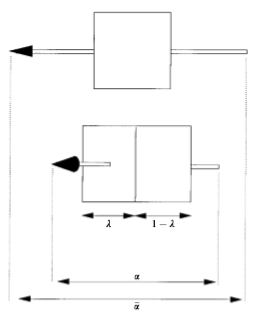
\includegraphics[width = 4cm, left]{Images/PointerSkize.PNG}
            \caption{Schematic pointer in Koenderink et al. (2000).}
            \label{schematicPointer}
        \end{figure}
    \end{minipage}
    \begin{minipage}{5cm}
        \begin{itemize}
            \item Exocentric pointing
            \item Natural conditions: open field, head movement
            \item Curvature dependent on distance $\Rightarrow$ non-constant curvature
            \item Elliptic in near space, hyperbolic in far space
        \end{itemize}
    \end{minipage}
\end{frame}

\begin{frame}{Hypotheses}
    \begin{itemize}
        \item Similar results to real life (RL) experiment
        \item Differences between the dark and the light condition
        \item Symmetry in the dark condition
        \item Angular deviation will depend on $\beta$
        
    \end{itemize}
\end{frame}

\section{Method}

\begin{frame}{Method}
    \begin{minipage}{6cm}
        \begin{figure}
            \centering
            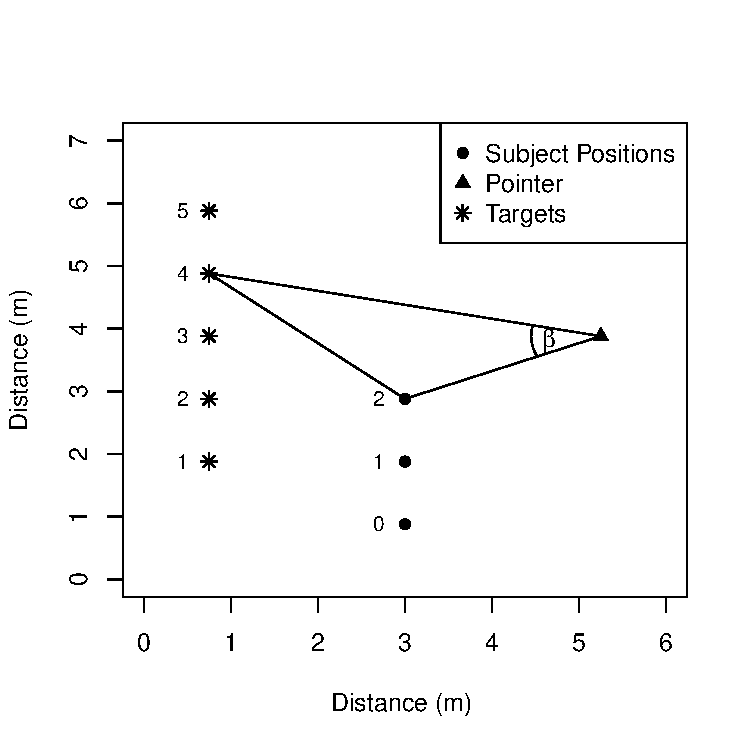
\includegraphics[width = 6cm]{Images/schematicAufbau.pdf}
            \caption{Schematic image of stimuli arrangement.}
            \label{schematicAufbau}
        \end{figure}
    \end{minipage}
    \begin{minipage}{5cm}
        \begin{itemize}
            \item Four (valid) subjects
            \item Additionally, one non-na\"{i}ve subject for comparison with RL experiment
        \end{itemize}
    \end{minipage}
\end{frame}

\begin{frame}{Method}
    \begin{minipage}{10cm}
        \begin{figure}
            \centering
            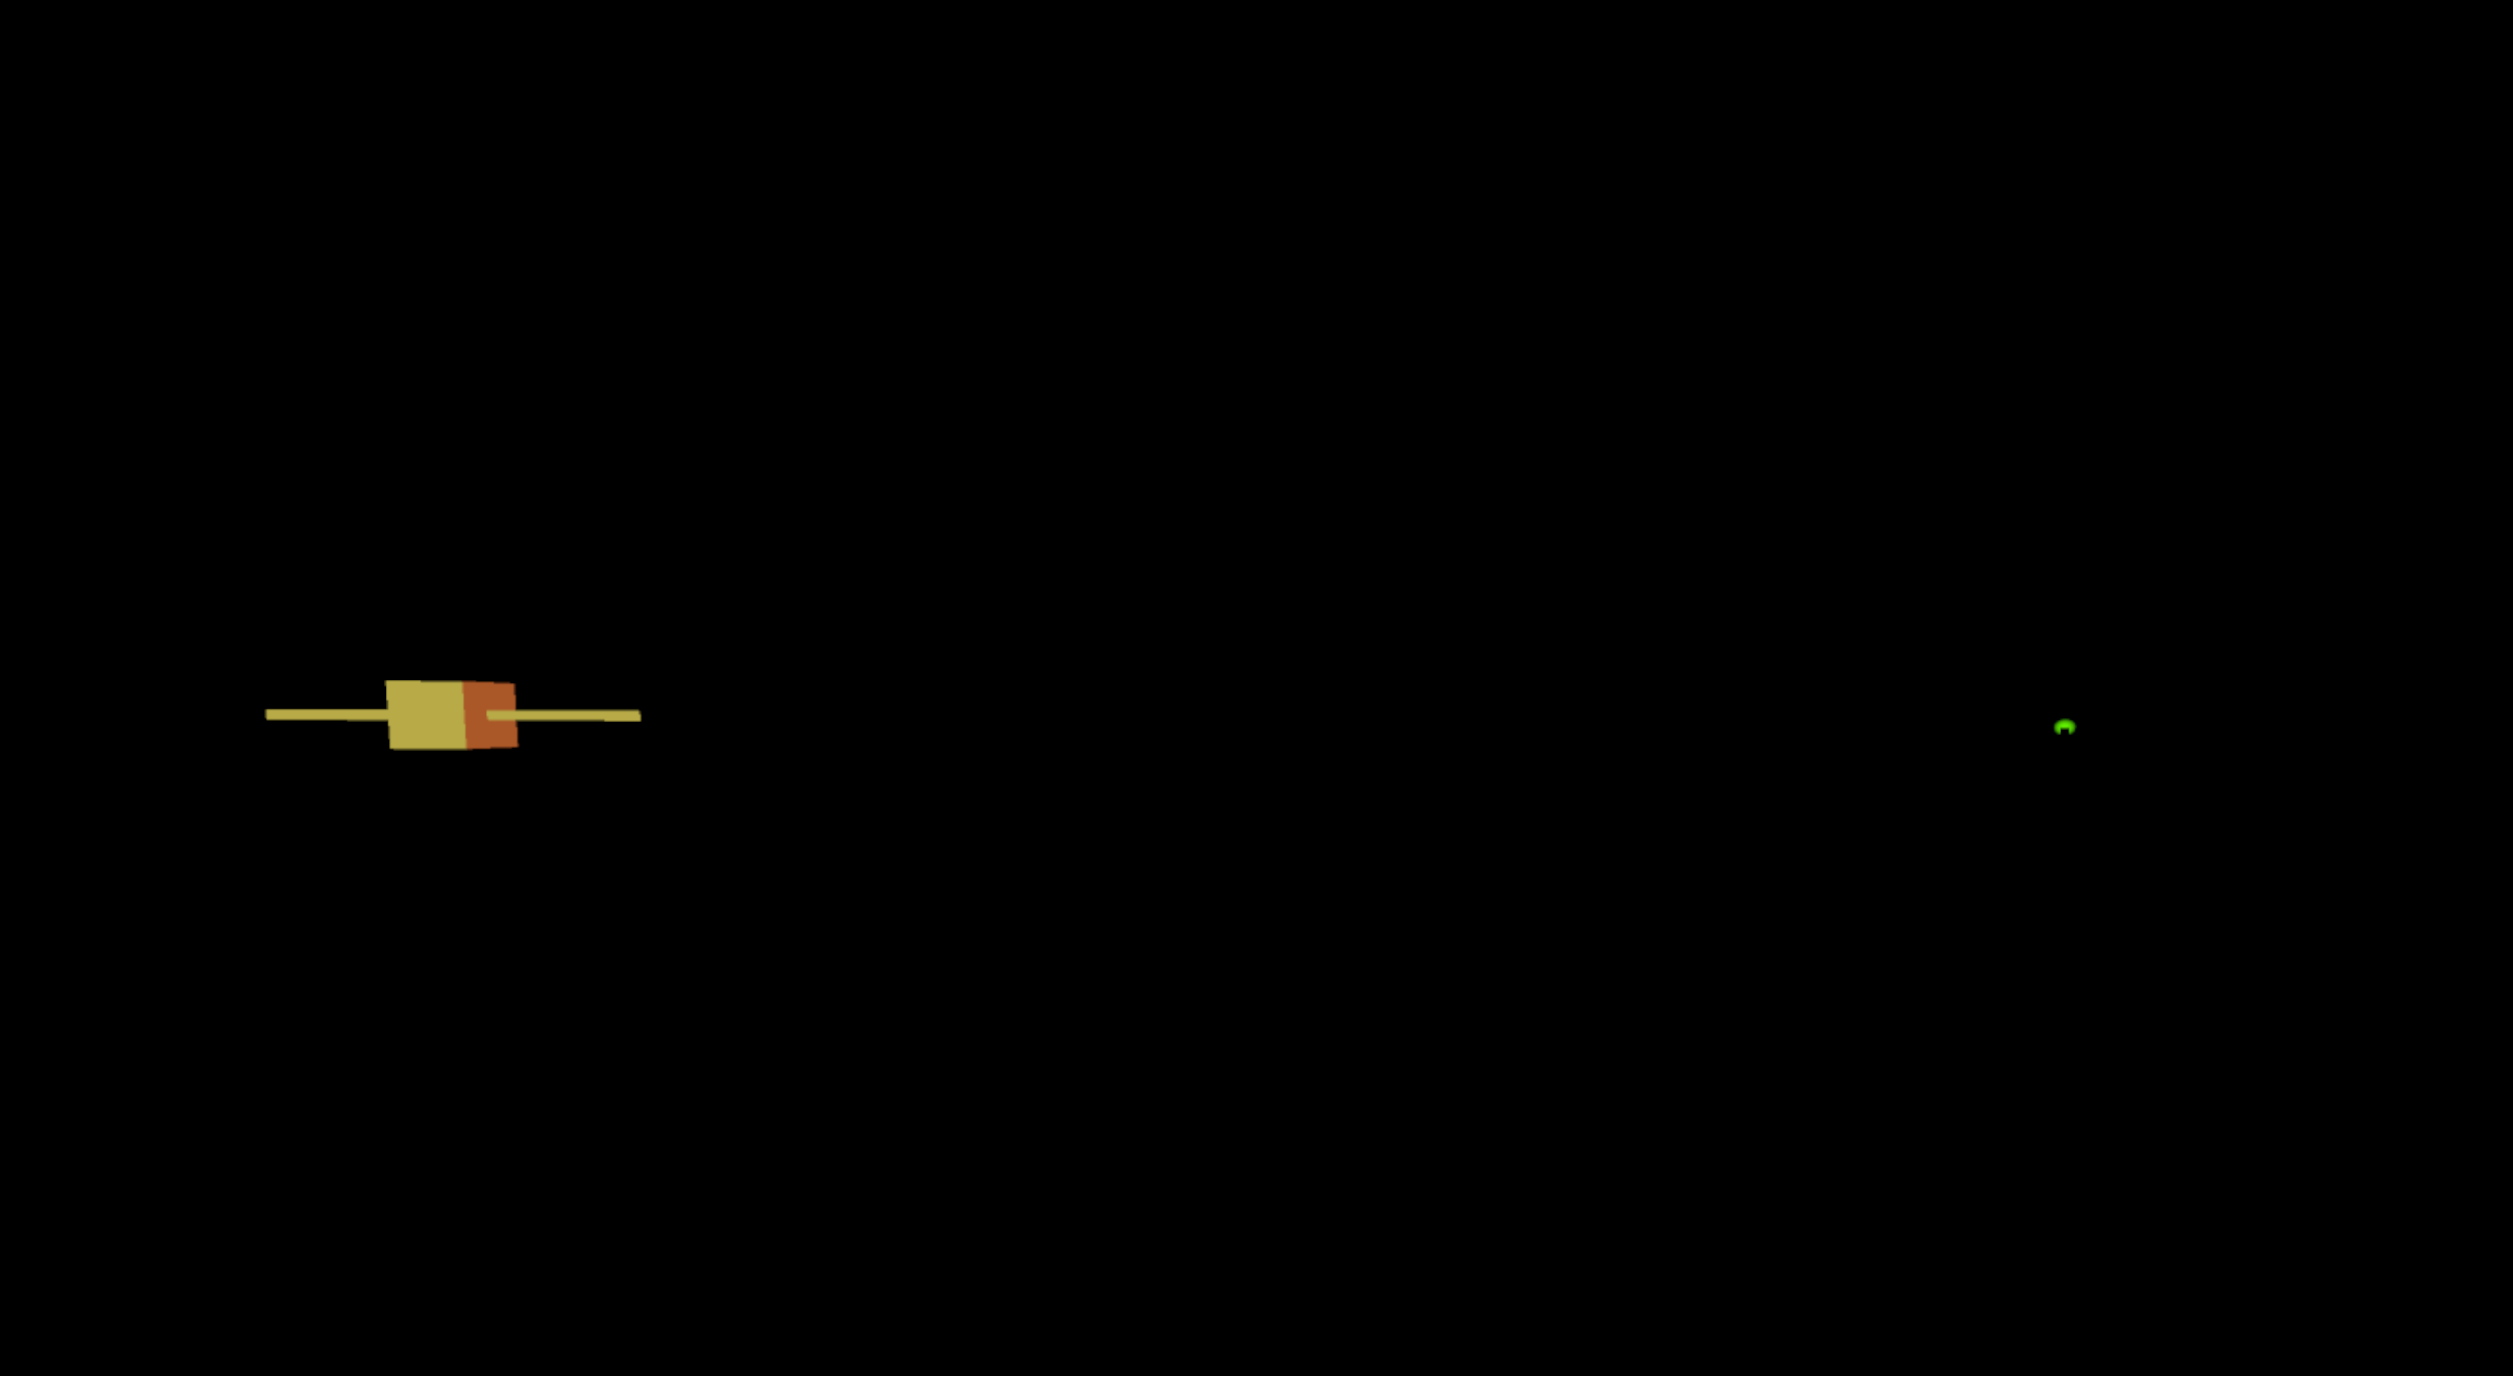
\includegraphics[width = 10cm]{Images/SzeneDunkelBeispiel.png}
            \caption{Example scene, dark condition.}
            \label{ExSzeneDark}
        \end{figure}
    \end{minipage}
\end{frame}

\begin{frame}{Method}
    \begin{minipage}{10cm}
        \begin{figure}
            \centering
            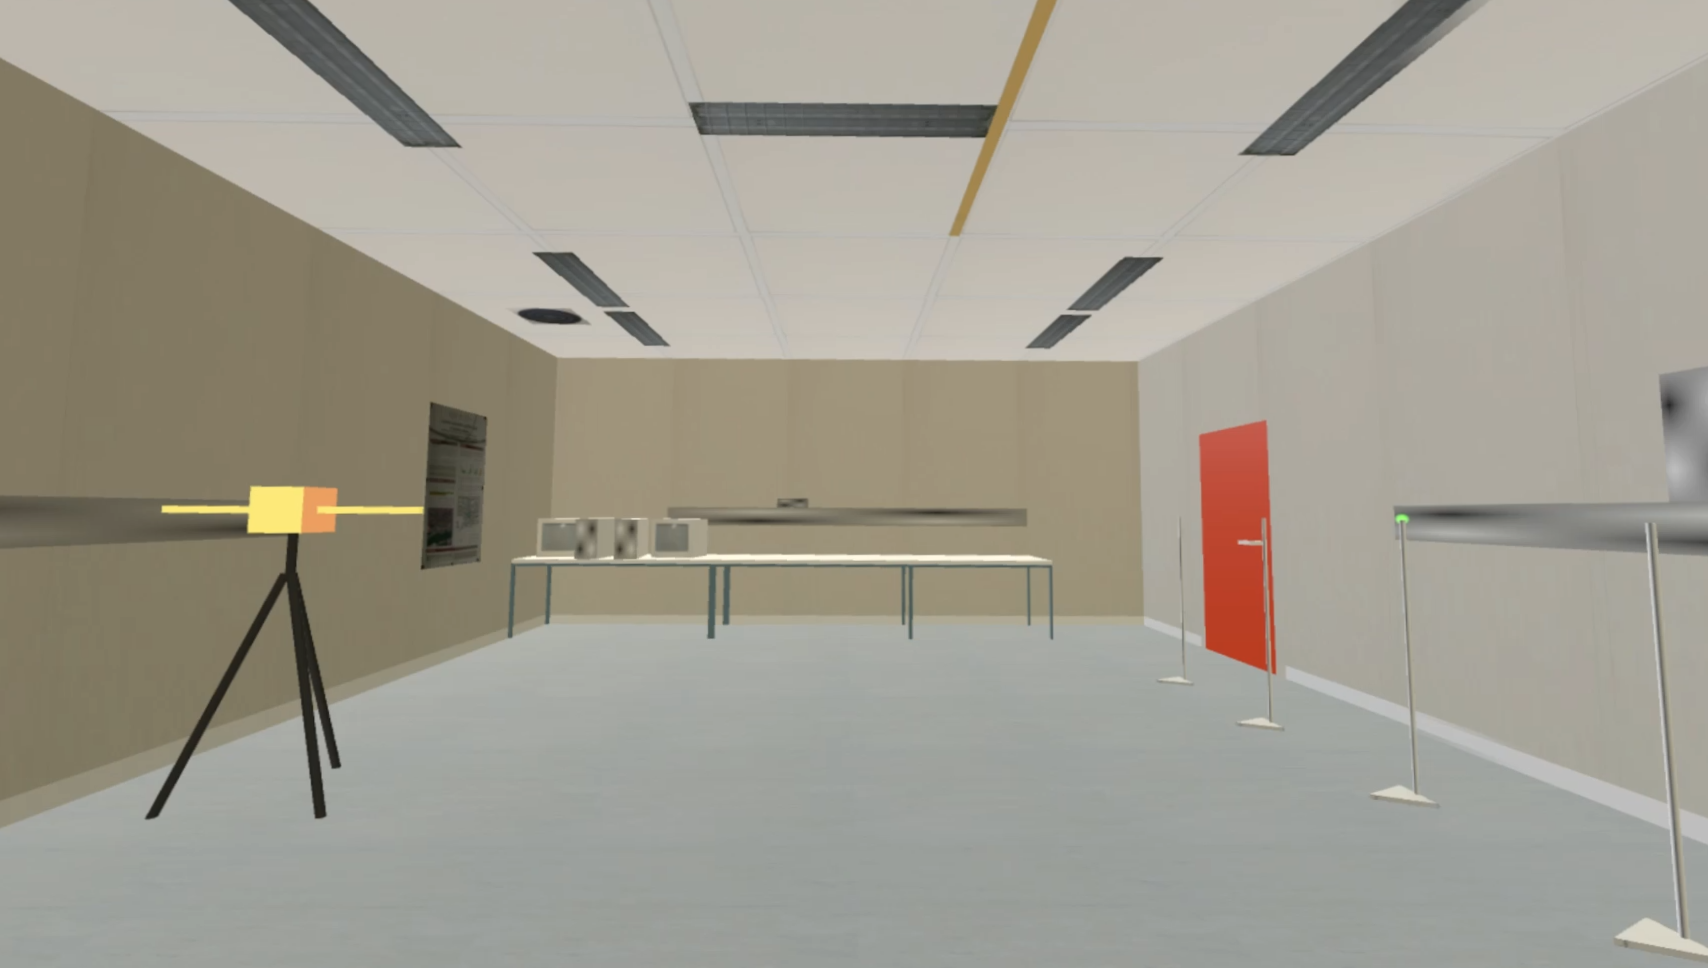
\includegraphics[width = 10cm]{Images/SzenenBeispiel.png}
            \caption{Example scene, light condition.}
            \label{ExSzeneLight}
        \end{figure}
    \end{minipage}
\end{frame}

\section{Results and Discussion}
\begin{frame}{Results and Discussion}
    \begin{itemize}
        \item Measured: pointer orientation, reaction time, head orientation 
        \item Intrinsic geometry depends on individual $\Rightarrow$ evaluation per subject
        \item ANOVA over: lighting, pointer position, $\beta$, subject position
    \end{itemize}
\end{frame}

\begin{frame}{Results and Discussion: $\beta$}
    \begin{minipage}{10cm}
        \begin{figure}
            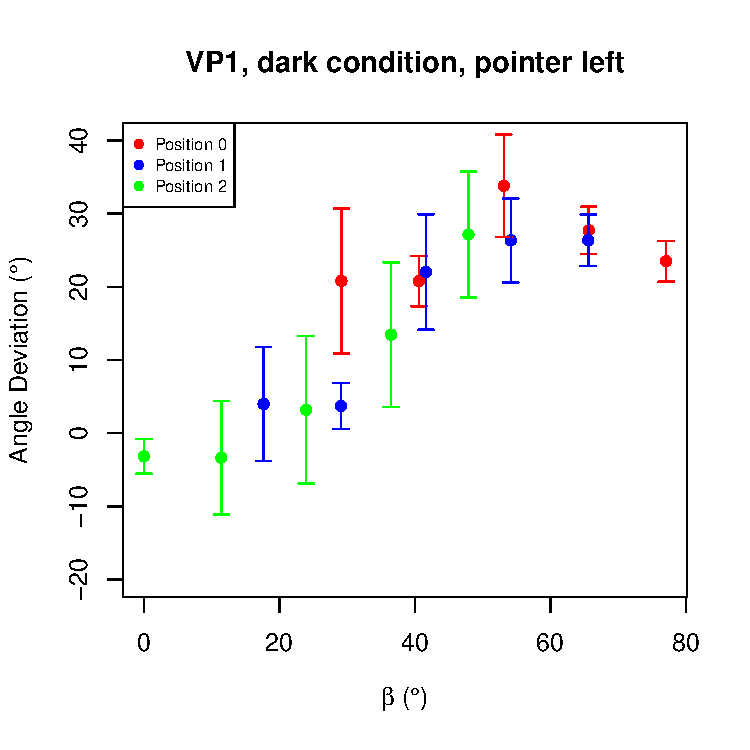
\includegraphics[clip, trim = 0cm 0.5cm 0.5cm 0.6cm, width = 3.8cm]{Images/plots/AngleDevVP1DarkLeft.pdf}
            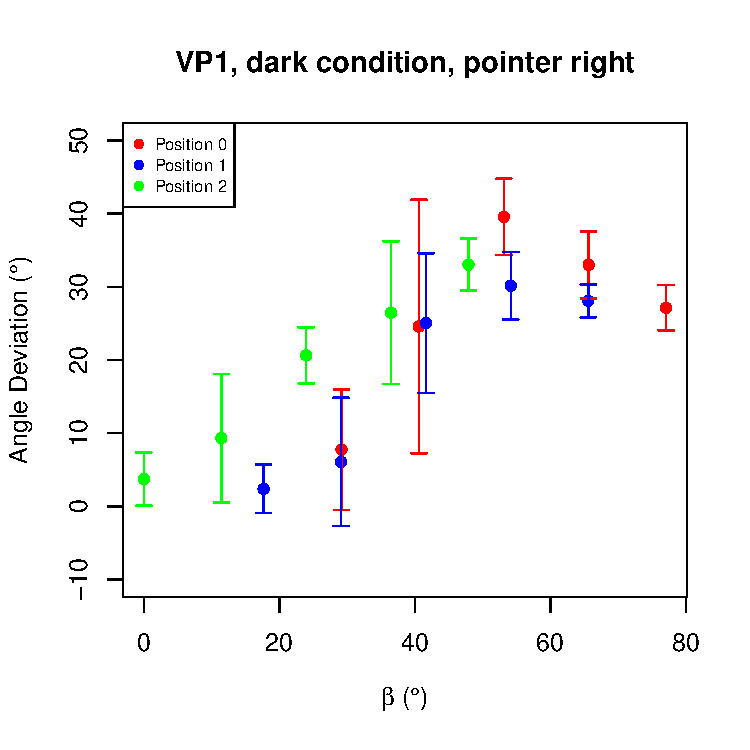
\includegraphics[clip, trim = 0cm 0.5cm 0.5cm 0.6cm, width = 3.8cm]{Images/plots/AngleDevVP1DarkRight.pdf}
            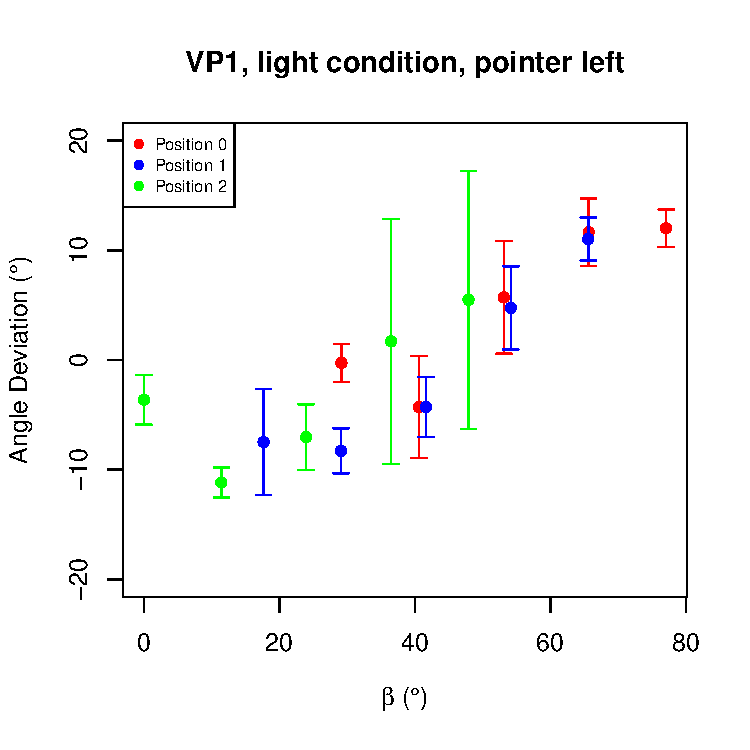
\includegraphics[clip, trim = 0cm 0.5cm 0.5cm 0.6cm, width = 3.8cm]{Images/plots/AngleDevVP1LightLeft.pdf}
            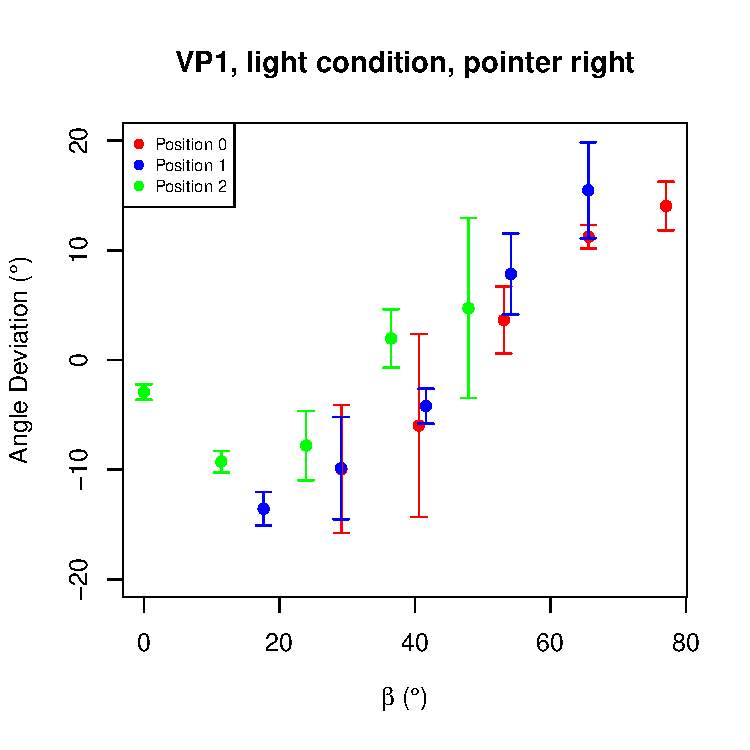
\includegraphics[clip, trim = 0cm 0.5cm 0.5cm 0.6cm, width = 3.8cm]{Images/plots/AngleDevVP1LightRight.pdf}
            \caption{Angular deviation first subject (VP1).}
            \label{DevVP1}
        \end{figure}
    \end{minipage}
\end{frame}

\begin{frame}{Results and Discussion: Lighting}
    \begin{itemize}
        \item Lighting very significant for the first and the third subject
        \item Higher positive deviation in the dark condition
        \item More symmetry given in the light condition
    \end{itemize}
\end{frame}

\begin{frame}{Results and Discussion: Lighting}
    \begin{minipage}{10cm}
        \begin{figure}
            \centering
            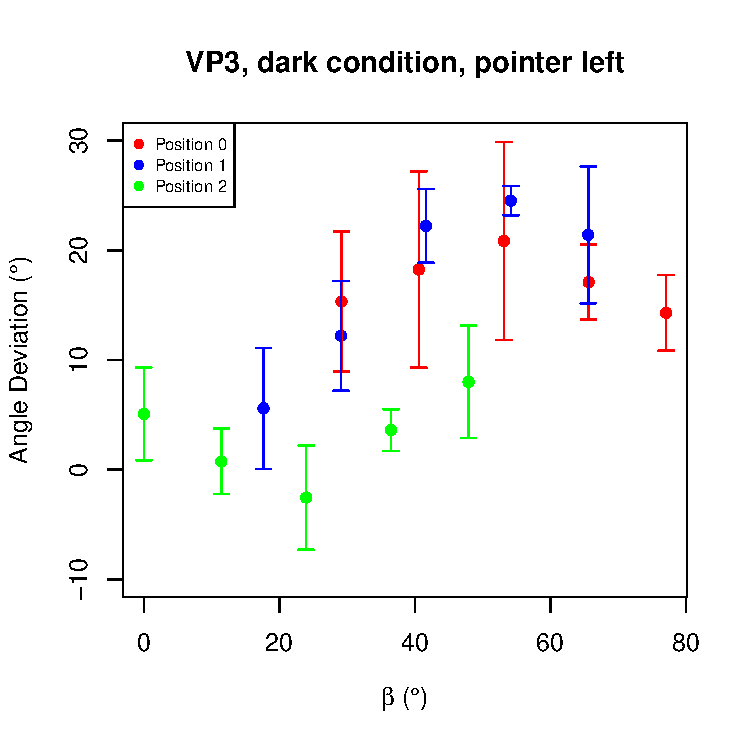
\includegraphics[clip, trim = 0cm 0.5cm 0.5cm 0.6cm, width = 3.8cm]{Images/plots/AngleDevVP3DarkLeft.pdf}
            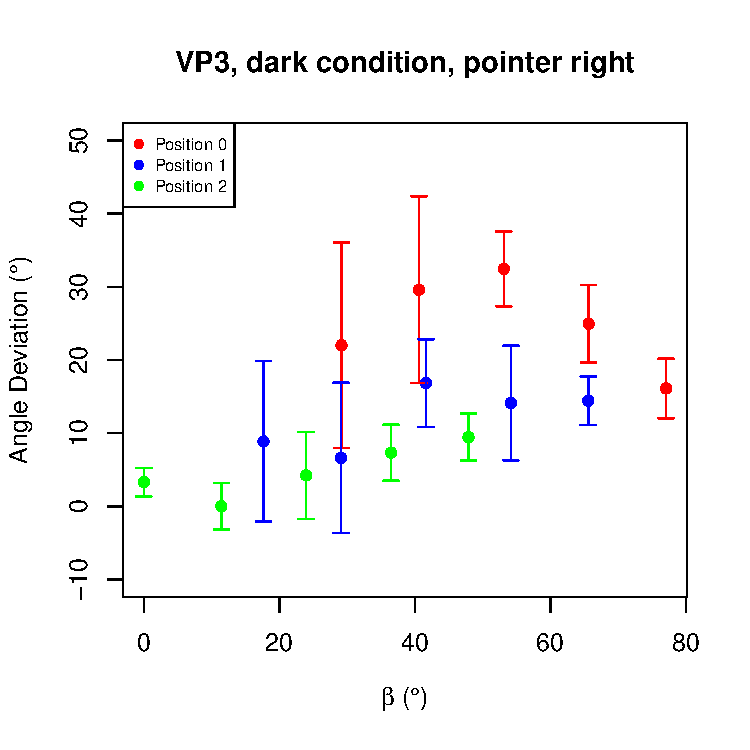
\includegraphics[clip, trim = 0cm 0.5cm 0.5cm 0.6cm, width = 3.8cm]{Images/plots/AngleDevVP3DarkRight.pdf}
            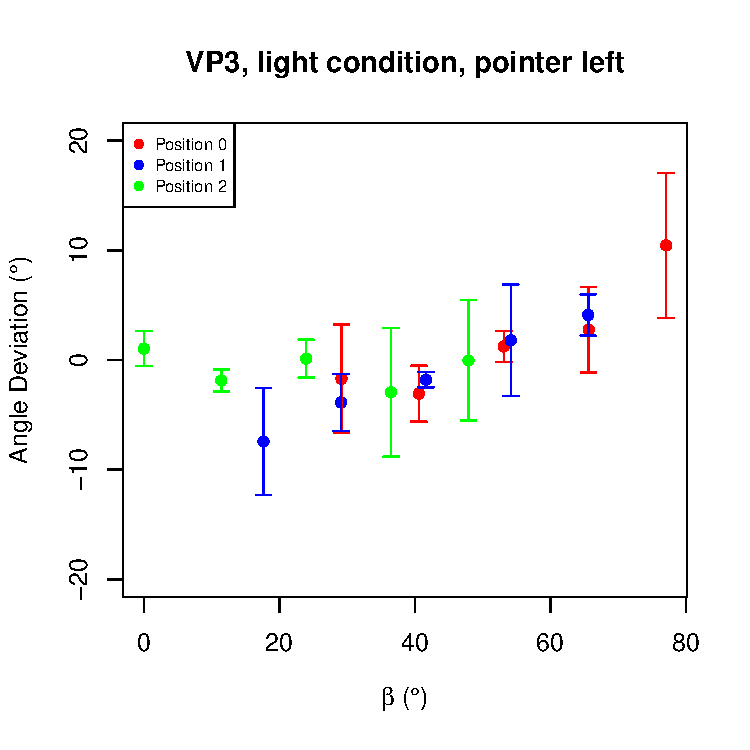
\includegraphics[clip, trim = 0cm 0.5cm 0.5cm 0.6cm, width = 3.8cm]{Images/plots/AngleDevVP3LightLeft.pdf}
            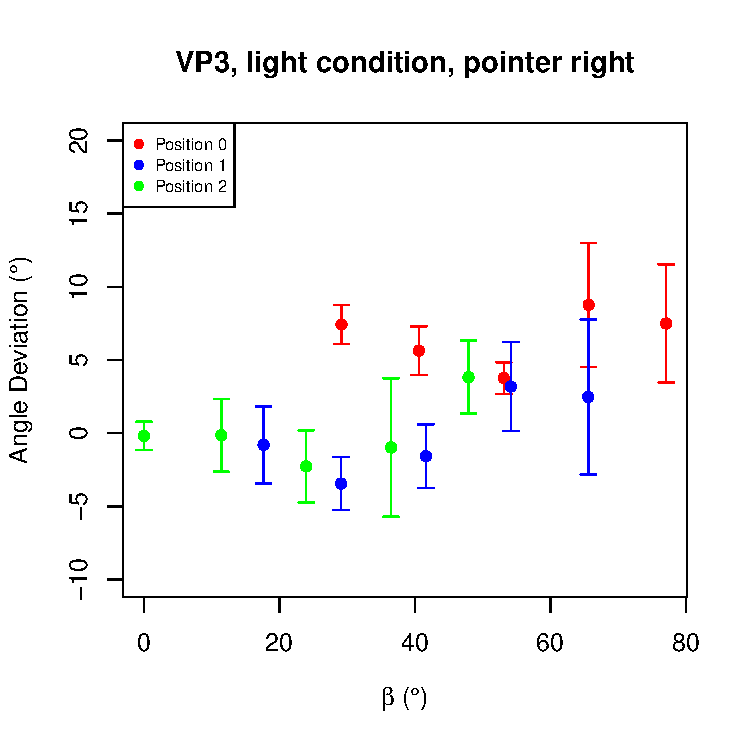
\includegraphics[clip, trim = 0cm 0.5cm 0.5cm 0.6cm, width = 3.8cm]{Images/plots/AngleDevVP3LightRight.pdf}
            \caption{Angular deviation third subject (VP3).}
            \label{DevVP3}
        \end{figure}
    \end{minipage}
\end{frame}

\begin{frame}{Results and Discussion: Symmetry}
    \begin{minipage}{10cm}
        \begin{figure}
            \centering
            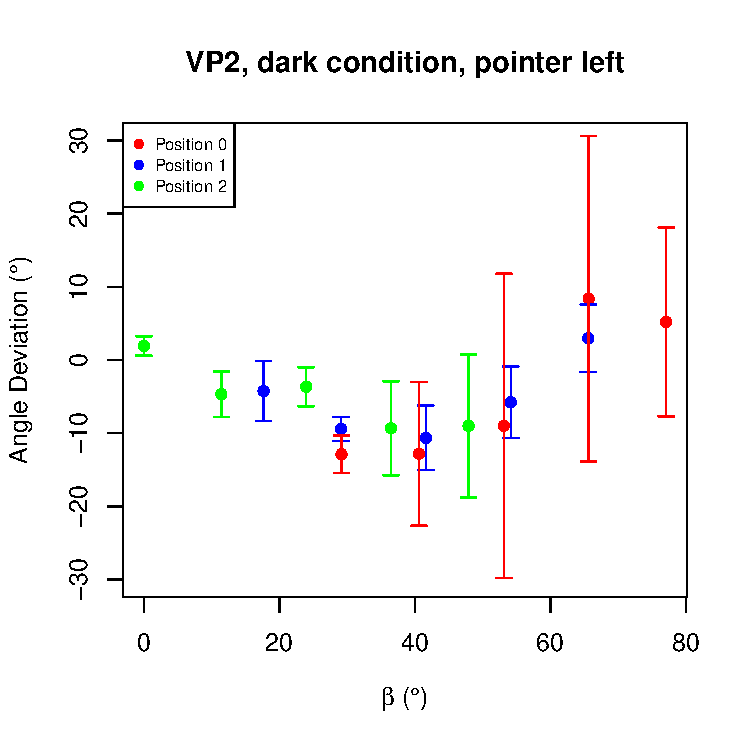
\includegraphics[clip, trim = 0cm 0.5cm 0.5cm 0.6cm, width = 3.8cm]{Images/plots/AngleDevVP2DarkLeft.pdf}
            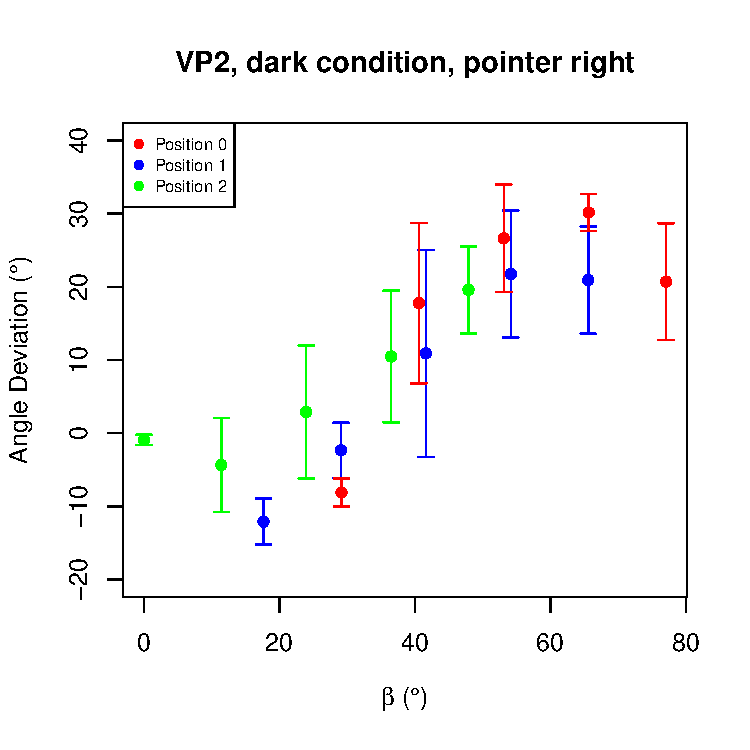
\includegraphics[clip, trim = 0cm 0.5cm 0.5cm 0.6cm, width = 3.8cm]{Images/plots/AngleDevVP2DarkRight.pdf}
            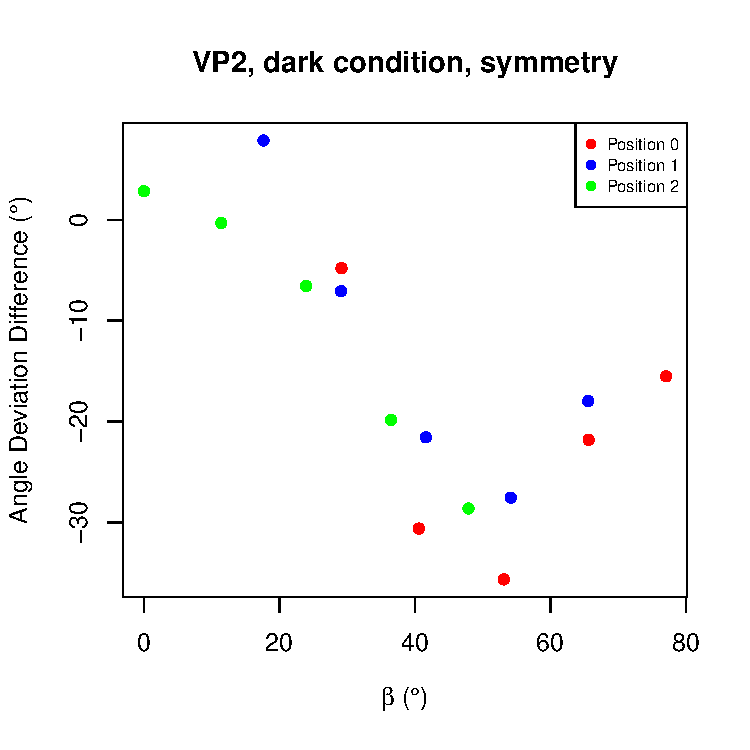
\includegraphics[clip, trim = 0cm 0.5cm 0.5cm 0.6cm, width = 3.8cm]{Images/plots/VP2Symmetry.pdf}
            \caption{Angular deviation second subject (VP2) in the dark condition and symmetry deviation (left pointer condition minus right pointer condition).}
            \label{DevVP2}
        \end{figure}
    \end{minipage}
\end{frame}


\begin{frame}{Results and Discussion: Subject Position}
    \begin{minipage}{12cm}
        \begin{figure}
            \centering
            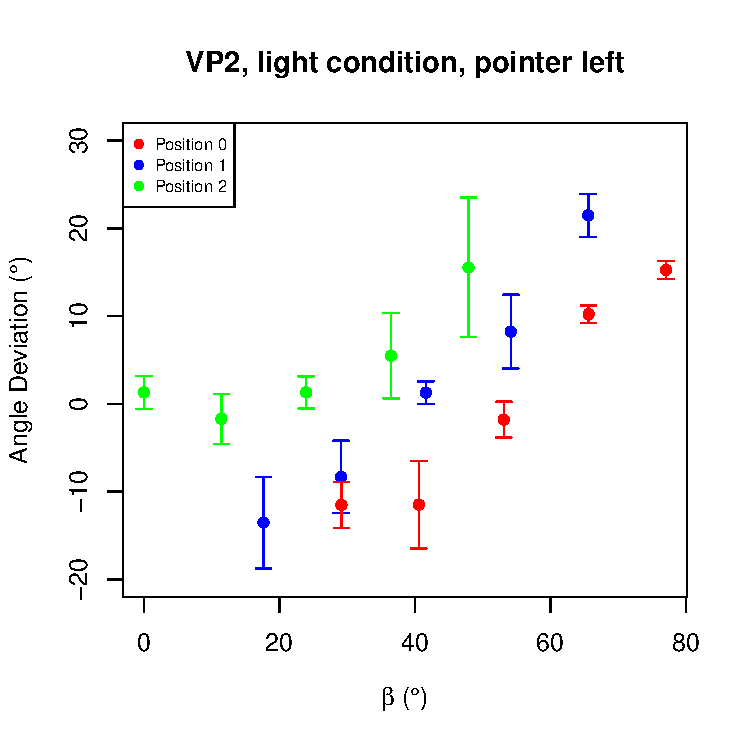
\includegraphics[clip, trim = 0cm 0.5cm 0.5cm 0.6cm, width = 3.8cm]{Images/plots/AngleDevVP2LightLeft.pdf}
            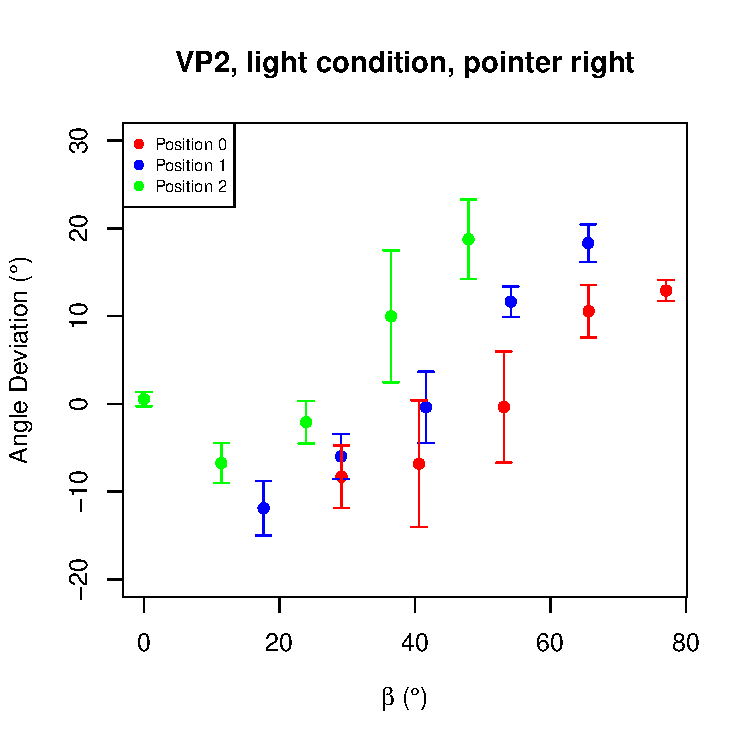
\includegraphics[clip, trim = 0cm 0.5cm 0.5cm 0.6cm, width = 3.8cm]{Images/plots/AngleDevVP2LightRight.pdf}\\
            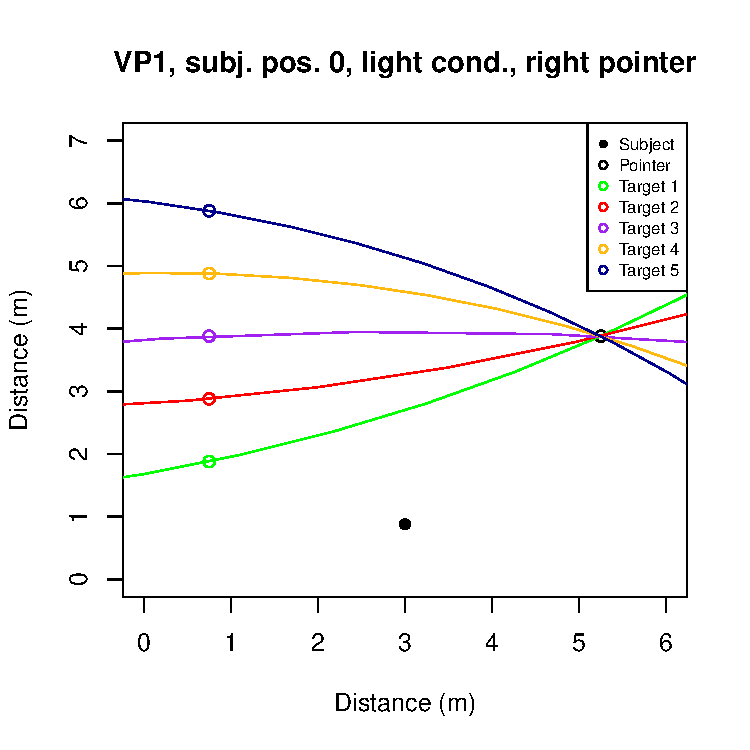
\includegraphics[clip, trim = 0.1cm 0.5cm 0.95cm 0.6cm, width=3.85cm]{Images/plots/VP1lightrightPos0Curves.pdf}
            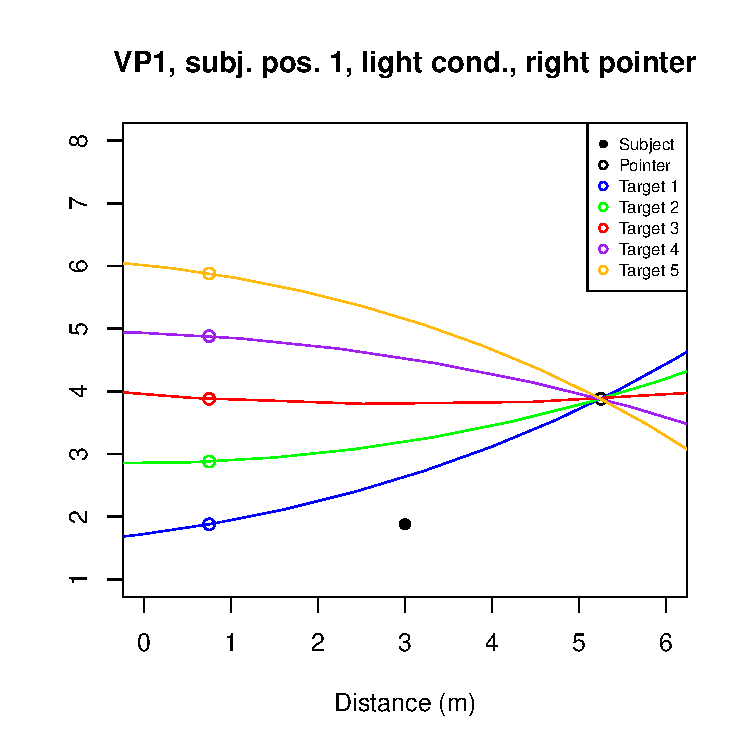
\includegraphics[clip, trim = 1.15cm 0.5cm 0.95cm 0.6cm, width=3.5cm]{Images/plots/VP1lightrightPos1Curves.pdf}
            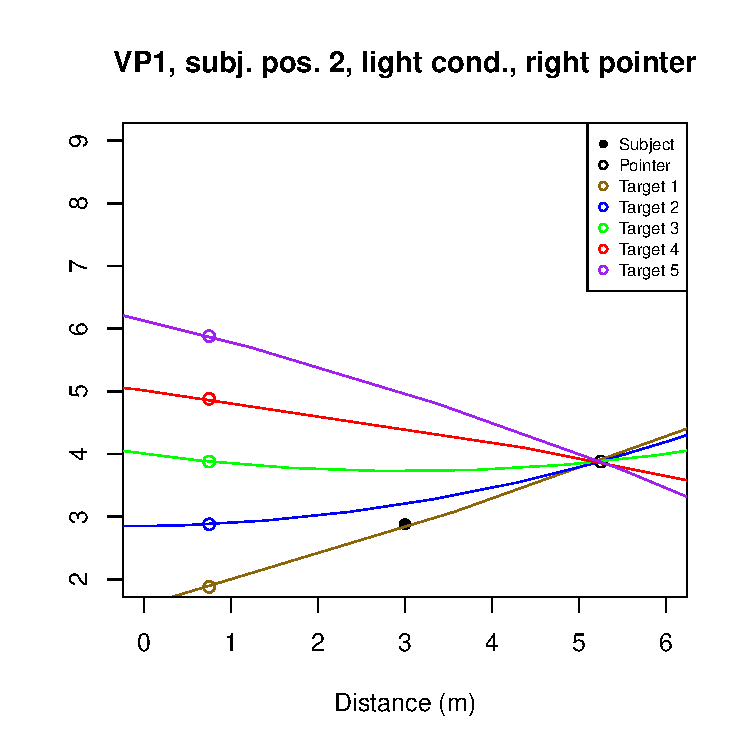
\includegraphics[clip, trim = 1.15cm 0.5cm 0.95cm 0.6cm, width=3.5cm]{Images/plots/VP1lightrightPos2Curves.pdf}
            \caption{Angular deviation second subject (VP2) in the light condition and circle arcs first subject (VP1) in the light condition, pointer right.}
            \label{DevVP2}
        \end{figure}
    \end{minipage}
\end{frame}

% \item Twelve blocks: Half dark, half light condition, half pointer left, half pointer right, each block subject at different position

\begin{frame}{Results and Discussion: Comparison VR with RL}
    \begin{minipage}{10cm}
        \begin{figure}
            \centering
            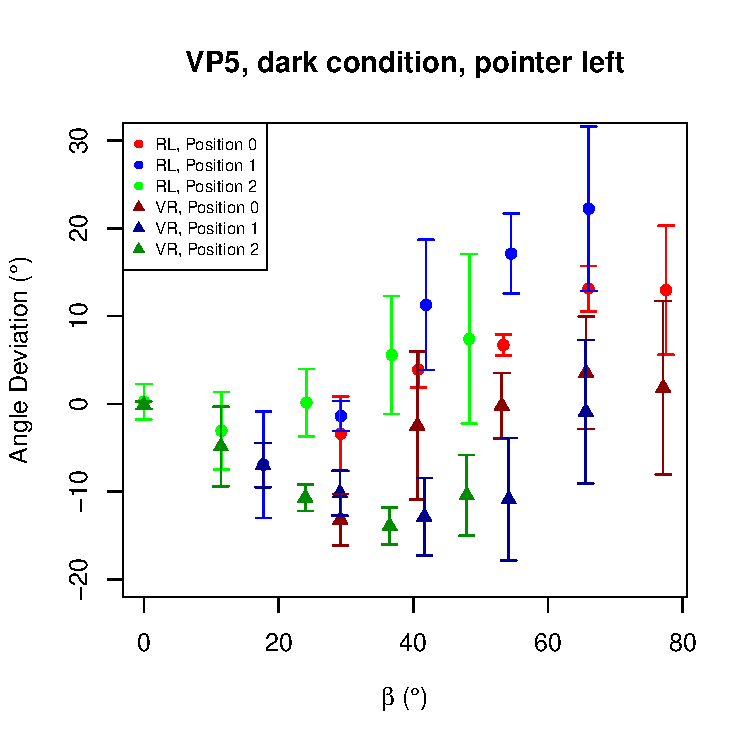
\includegraphics[clip, trim = 0cm 0.5cm 0.5cm 0.6cm, width = 3.8cm]{Images/plots/AngleDevVP5BOTHDarkLeft.pdf}
            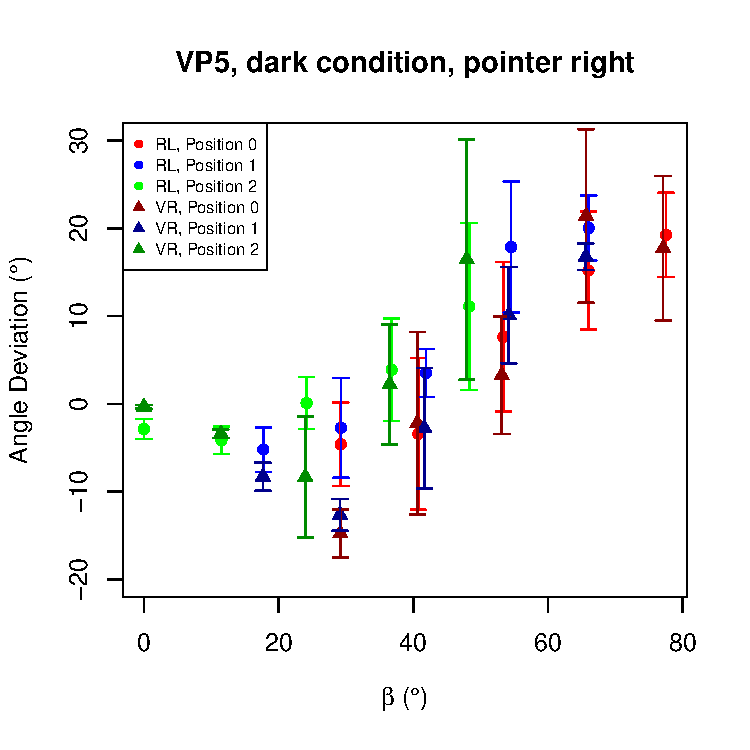
\includegraphics[clip, trim = 0cm 0.5cm 0.5cm 0.6cm, width = 3.8cm]{Images/plots/AngleDevVP5BOTHDarkRight.pdf}
            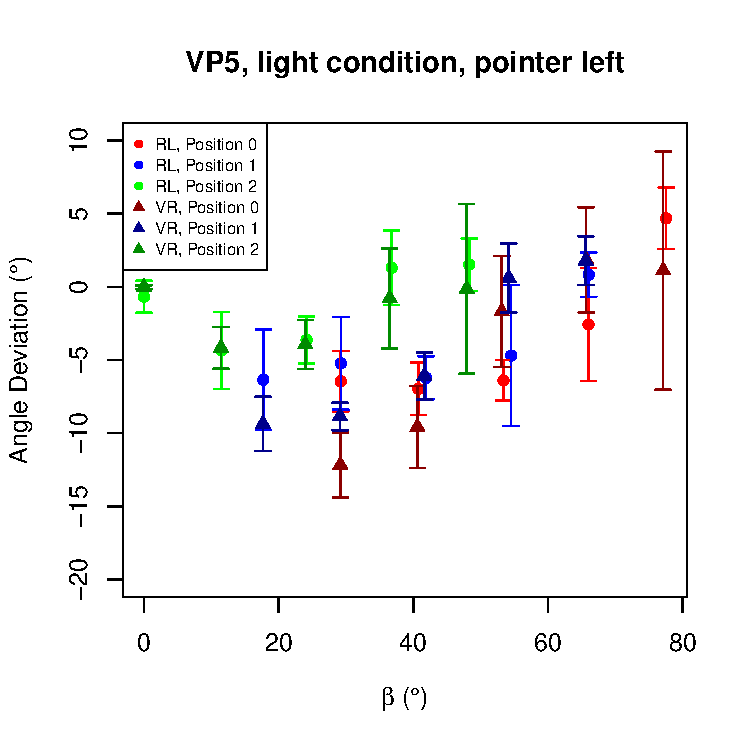
\includegraphics[clip, trim = 0cm 0.5cm 0.5cm 0.6cm, width = 3.8cm]{Images/plots/AngleDevVP5BOTHLightLeft.pdf}
            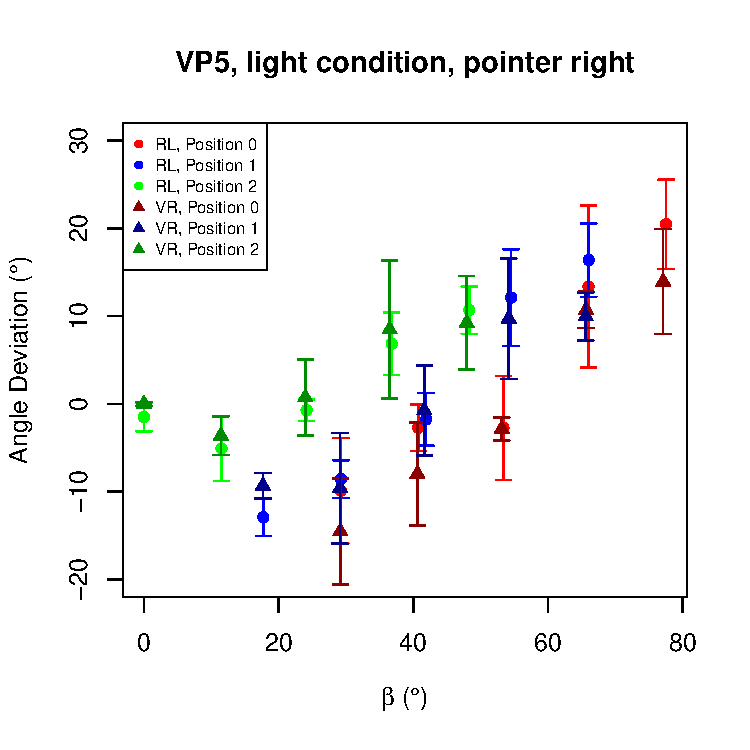
\includegraphics[clip, trim = 0cm 0.5cm 0.5cm 0.6cm, width = 3.8cm]{Images/plots/AngleDevVP5BOTHLightRight.pdf}
            \caption{Angular deviation real life experiment (RL) and virtual reality experiment (VR) fifth subject (VP5).}
            \label{DevVP3}
        \end{figure}
    \end{minipage}
\end{frame}

\begin{frame}{Conclusion}
    \begin{itemize}
        \item Intrinsic geometry of the visual space is of non-constant curvature 
        \item Lighting and hence monocular cues make a difference
        \item VR is a possible method for measuring the intrinsic geometry of the visual space
    \end{itemize}
\end{frame}

\section{Conclusion}

\begin{frame}{}
    \large{Thank you for your attention! :)}
\end{frame}
\end{document}
